\chapter[Matematická analýza]{Matematická analýza}
\label{matematicka_analyza} % id kapitoly pre prikaz ref

\section{Limita reálnej funkcie jednej reálnej premennej}
\subsection{definícia vlastnej a nevlastnej limity}
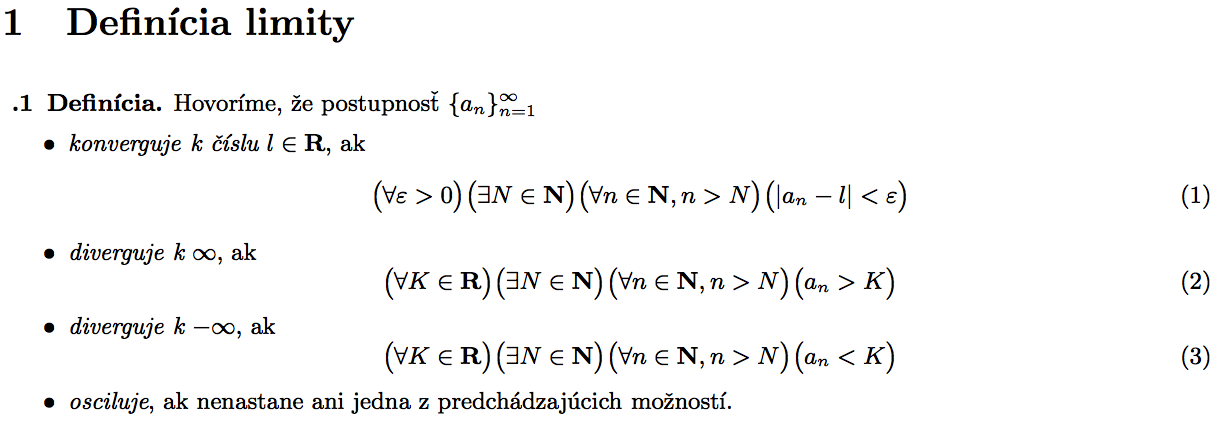
\includegraphics[width=1\textwidth]{images/analyza/def_lim}\\
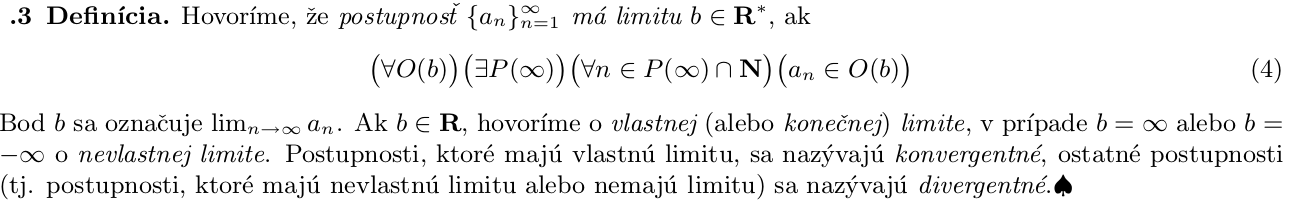
\includegraphics[width=1\textwidth]{images/analyza/def_nev_lim}\\
\subsection{vety o výpočte limít}
\subsection{číslo e}
\subsection{Cauchyho-Bolzanovo kritérium konvergencie postupnosti}


\section{Spojité funkcie a ich základné vlastnosti}
\subsection{definícia spojitej funkcie}
\subsection{Darbouxova vlastnosť}
\subsection{vlastnosti spojitých funkcií na uzavretých ohraničených intervaloch}

\section{Derivácia funkcie a jej využitie na vyšetrovanie priebehu funkcie}
\subsection{definícia derivácie}
\subsection{vety o výpočte derivácií}
\subsection{vety o strednej hodnote}
\subsection{derivácie vyšších rádov}
\subsection{vyšetrovanie monotónnosti}
\subsection{extrémov a konvexnosti pomocou derivácií}


\section{Primitívna funkcia a neurčitý integrál}
\subsection{definícia neurčitého integrálu}
\subsection{metóda per partes a substitúcie}
\subsection{univerzálna trigonometrická substitúcia}


\section{Riemannov určitý integrál}
\subsection{definícia riemannovsky integrovateľnej funkcie}
\subsection{integrovateľnosť monotónnych a spojitých funkcií}
\subsection{Newtonov-Leibnizov vzorec}
\subsection{integrál ako funkcia hranice}


\section{Číselné rady}
\subsection{definícia číselného radu}
\subsection{Cauchyho-Bolzanovo kritérium konvergencie radu}
\subsection{kritériá pre konvergenciu radov s nezápornými členmi}
\subsection{Leibnizovo kritérium}
\subsection{relatívne a absolútne konvergentné rady}
\subsection{prerovnanie radov}


\section{Mocninové a Taylorove rady}
\subsection{definícia mocninového radu}
\subsection{polomer a interval konvergencie}
\subsection{derivovanie a integrovanie mocninových radov}
\subsection{definícia Taylorovho radu}
\subsection{pojem analytickej funkcie}


